\def \statemodule {MotionEstimation}
\def \handleevent {Алгоритм обработки событий}

\section{Проектирование программного средства}
\subsection{Датчики}
В качестве поддерживаемых датчиков было выбрано три ключевых:
\begin{itemize}
	\item 2D Lidar;
	\item IMU;
	\item GPS.
\end{itemize}

Эти датчики обеспечивают систему данными о пространстве, в котором находится
робот, его ориентации и глобальном местоположении.
2D Lidar позволяет получать информацию о препятствиях вокруг устройства, IMU
предоставляет данные о наклоне и угловых ускорениях, а GPS -- о глобальной
позиции робота. Все эти данные интегрируются в систему навигации, создавая
основу для безопасного и эффективного перемещения устройства в различных
условиях.

2D Lidar (Light Detection and Ranging) работает на основе принципа измерения
расстояния до объектов с использованием лазерных импульсов. Ли дар излучает
лазерные импульсы, которые отражаются от объектов, встречающих их на пути.
Время, которое требуется импульсу для прохождения от лидара до объекта и
обратно, используется для вычисления расстояния до объекта. Этот процесс
повторяется многократно по всей области сканирования, создавая карту расстояний
на основе измерений.

\begin{figure}[h]
\centering
	\fbox{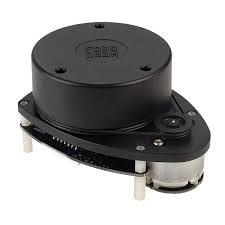
\includegraphics[width=9cm]{2d_lidar}}
\caption{2D Lidar}
\end{figure}

2D лидары обычно работают в плоскости, что означает, что они измеряют расстояния
только в одном направлении (по горизонтали или вертикали). Сканер вращается или
перемещается по оси, чтобы покрыть широкую область, создавая двумерное
изображение окружающего пространства. С помощью таких данных система может
строить карту и распознавать объекты, определяя их положение и расстояние до
них, что крайне важно для навигации роботов и беспилотных автомобилей.

IMU (Inertial Measurement Unit) -- это датчик, который измеряет и сообщает
информацию о движении и ориентации объекта в пространстве. Он состоит из трех
основных компонентов: акселерометров, гироскопов и иногда магнитометров.
Акселерометры измеряют ускорения по трем осям (X, Y, Z), что позволяет
определить изменение скорости и положение объекта относительно земной
гравитации. Гироскопы отслеживают угловые скорости вращения вокруг тех же осей,
что помогает измерять ориентацию объекта и его вращения. Магнитометры, если они
присутствуют, измеряют магнитное поле Земли, что позволяет дополнительно
корректировать ориентацию.

Принцип работы IMU заключается в интеграции данных с этих сенсоров, чтобы
получить полное представление о движении и положении объекта. Например,
акселерометры могут обнаружить, если устройство наклоняется или ускоряется, а
гироскопы отслеживают угловые изменения, такие как вращение вокруг своей оси.
Это позволяет системе вычислить изменения ориентации и траекторию движения, что
полезно в таких приложениях, как робототехника, авиация и навигация в условиях
отсутствия GPS.

GPS -- это навигационная система, основанная на использовании спутников для
определения местоположения объектов на Земле. Система состоит из спутников,
находящихся на орбите, наземных станций и приемников, которые используются для
получения данных о местоположении. Спутники передают сигналы с точным временем,
и приемник на Земле, получая эти сигналы от нескольких спутников, может
вычислить свое местоположение.

Принцип работы GPS заключается в измерении времени, которое требуется сигналу,
чтобы добраться от спутника до приемника. Поскольку спутники известны своей
точной орбитой, приемник может определить расстояние до каждого спутника,
используя это время. Получая сигналы от как минимум четырех спутников, приемник
может точно вычислить свою абсолютную позицию в трехмерном пространстве --
определяя широту, долготу и высоту, а также время. Эти данные обеспечивают
высокую точность определения местоположения, что критически важно для навигации
и локализации в реальном времени.

\subsection{CSM}
Correlative scan matching (CSM) -- это метод регистрации сканов лидара,
используемый в робототехнике для определения относительного положения робота на
карте. Его ключевое преимущество -- устойчивость к локальным минимумам и высокая точность, что делает его критически важным для задач одновременной локализации и построения карт (SLAM).

Принцип работы CSM заключается в поиске оптимального преобразования (сдвига и поворота) между двумя наборами точек (сканами), при котором достигается максимальное совпадение между ними. В отличие от итеративных методов, таких как ICP (Iterative Closest Point), которые зависят от начального приближения и могут застревать в локальных оптимумах, CSM осуществляет дискретный перебор возможных трансформаций в заданном диапазоне. Для каждой трансформации вычисляется функция качества совпадения, основанная на вероятностной модели окружающей среды или на карте стоимости.

Алгоритм строит карту стоимости, где каждой точке пространства соответствует значение, отражающее вероятность её принадлежности к объекту или свободному пространству. Затем, перебирая множество вариантов сдвигов и поворотов, CSM вычисляет суммарную оценку совпадения между текущим сканом и картой. Оптимальное преобразование выбирается как то, при котором эта оценка максимальна.

Преимущества CSM включают:
\begin{itemize}
	\item глобальный поиск решения, минимизирующий риск сходимости к локальным минимумам;
	\item высокую устойчивость к шуму и ошибкам сенсорных данных;
	\item возможность работы при значительной начальной неопределённости положения.
\end{itemize}

CSM широко применяется в задачах одновременной локализации и построения карт (SLAM), особенно для коррекции ошибок одометрии и закрытия петель, что позволяет значительно повысить точность и надёжность навигационных систем мобильных роботов.

\subsection{ICP}
Iterative Closest Point (ICP) -- это классический алгоритм регистрации облаков
точек, широко используемый в компьютерном зрении и робототехнике для точного
выравнивания двух наборов данных, полученных с помощью лидаров или других
3D-сканеров.

Основная цель ICP -- минимизировать расстояние между двумя облаками точек:
фиксированным эталонным (reference) и подвижным (source), который необходимо
трансформировать (сдвинуть и повернуть) так, чтобы максимально приблизить к
эталону. Алгоритм работает итеративно, последовательно уточняя параметры
преобразования.

\subsubsection{Принцип работы ICP}

1 Алгоритм начинается с предварительной оценки преобразования, которое
приблизительно совмещает исходное облако с эталонным. Качество начального
приближения существенно влияет на результат, поскольку ICP может сойтись к
локальному минимуму.
    
2 Для каждой точки подвижного облака находится ближайшая точка в эталонном
облаке по евклидову расстоянию. Для ускорения поиска обычно используется
структура данных k-d дерево.
    
3 На основе найденных пар точек вычисляется оптимальное преобразование (смещение
и поворот), минимизирующее среднеквадратичное расстояние между соответствующими
точками. Часто применяется метод наименьших квадратов.
    
4 Подвижное облако точек трансформируется с использованием найденного
преобразования.
    
5 Шаги поиска соответствий и оценки преобразования повторяются до тех пор, пока
изменение ошибки не станет меньше заданного порога или не будет достигнуто
максимальное число итераций.

\subsubsection{Особенности и ограничения}
\begin{itemize}
	\item ICP чувствителен к качеству начального приближения и может застревать в локальных оптимумах;
	\item алгоритм хорошо работает при небольших смещениях и поворотах между сканами;
	\item существует множество вариантов ICP, включая point-to-point (точка к точке) и point-to-plane (точка к плоскости), последний из которых лучше подходит для структурированных поверхностей;
	\item ICP широко применяется для локализации роботов, построения карт, сшивки 3D-моделей и коррекции ошибок одометрии.
\end{itemize}

ICP является базовым инструментом для регистрации 2D и 3D данных в задачах SLAM, реконструкции объектов и навигации мобильных платформ, особенно когда требуется точное совмещение облаков точек, полученных с разных позиций или в разное время.

Таким образом, ICP -- это эффективный и относительно простой алгоритм, обеспечивающий точное выравнивание облаков точек за счёт итеративного уточнения преобразования между ними.

В алгоритме Iterative Closest Point (ICP) задача сводится к поиску оптимального жёсткого преобразования (поворота и сдвига), которое минимизирует сумму квадратов расстояний между соответствующими точками двух облаков. Для решения этой задачи на каждом шаге, когда соответствия между точками уже известны, широко применяется метод сингулярного разложения матриц (SVD, Singular Value Decomposition).


\subsection{Описание модулей системы}

\subsection{Карты}


\subsection{Язык программирования}
Robot Operating System (ROS) представляет собой широко используемую программную
платформу для разработки робототехнических систем, и одной из её ключевых
особенностей является то, что она написана на языке программирования C++. Этот
выбор не случаен: C++ считается стандартом индустрии благодаря своей высокой
производительности, гибкости и возможности работы на низком уровне с аппаратным
обеспечением. В контексте робототехники, где требуется быстрая обработка данных
с датчиков и управление механизмами в реальном времени, такие качества C++
становятся незаменимыми. Использование C++ в ROS позволяет разработчикам
создавать эффективные и масштабируемые решения для сложных задач, таких как
автономная навигация, обработка сигналов или взаимодействие с физическими
устройствами. Этот язык обеспечивает тонкий контроль над ресурсами системы, что
особенно важно для мобильных платформ с ограниченными вычислительными
мощностями. Кроме того, C++ обладает богатым набором библиотек и инструментов,
которые упрощают интеграцию ROS с другими технологиями, укрепляя его как
стандарта в индустрии робототехники.

Несмотря на все преимущества C++ как стандарта индустрии и основы для ROS, в
последние годы всё большее внимание в разработке программного обеспечения,
включая робототехнику, привлекает язык программирования Rust. В контексте ROS
уже появляются инициативы по интеграции Rust, что может дополнить или даже со
временем частично заменить C++, предлагая разработчикам более надёжный и удобный
инструмент для создания автономных систем, сохраняя при этом совместимость с
существующей экосистемой ROS.

Одним из ключевых преимуществ Rust является его способность обеспечивать
безопасность многозадачности. В отличие от C++, который требует дополнительных
усилий для безопасного выполнения параллельных операций, Rust изначально
предусматривает механизмы предотвращения гонок данных, что делает код более
надежным. Это особенно важно для системы навигации, где необходимо параллельно
обрабатывать данные с различных сенсоров и вычислять управляющие команды без
риска возникновения ошибок синхронизации.

Rust также предоставляет встроенные инструменты для работы с асинхронным
программированием, что позволяет эффективно организовать обработку данных в
реальном времени. Асинхронные операции позволяют системе собирать данные с
сенсоров, планировать маршрут и управлять моторами без блокировки основного
потока выполнения, что способствует повышению производительности и снижению
задержек.

Программная экосистема Rust активно развивается, и существует множество
библиотек, которые могут быть использованы для решения задач, связанных с
обработкой сенсорных данных, математическими расчетами и оптимизацией маршрутов.
Это позволяет разработчикам легко интегрировать необходимые инструменты и
сокращать время на разработку и тестирование системы. Также, благодаря хорошей
поддержке со стороны сообщества, Rust предоставляет разработчикам множество
ресурсов для быстрого решения возникающих вопросов.

Ключевым преимуществом Rust является его кроссплатформенность. Код, написанный
на этом языке, может быть скомпилирован для различных платформ, что делает Rust
отличным выбором для мобильных роботов, которые могут работать на разных типах
оборудования. Это позволяет без значительных усилий адаптировать систему под
разные архитектуры и аппаратные платформы.

Будущие улучшения системы могут включать в себя добавление новых сенсоров,
улучшение алгоритмов SLAM и маршрутизации, а также интеграцию с внешними
системами, такими как онлайн-карты или системы для прогнозирования дорожной
ситуации. Rust, благодаря своей гибкости и безопасному управлению памятью,
идеально подходит для такой работы, обеспечивая долгосрочную устойчивость и
развитие проекта.

Таким образом, проектирование программного обеспечения для системы мобильной
навигации с использованием сенсоров и алгоритмов SLAM требует тщательной
проработки архитектуры, выбора эффективных технологий и инструментов. Язык Rust
является отличным выбором для разработки таких систем, благодаря своим
преимуществам в безопасности, производительности и поддержке многозадачности,
что делает его идеальным для создания высоконадежных и высокопроизводительных
приложений для робототехники.

Robot Operating System (ROS) представляет собой широко используемую программную
платформу для разработки робототехнических систем, и одной из её ключевых
особенностей является то, что она написана на языке программирования C++. Этот
выбор не случаен: C++ считается стандартом индустрии благодаря своей высокой
производительности, гибкости и возможности работы на низком уровне с аппаратным
обеспечением. В контексте робототехники, где требуется быстрая обработка данных
с датчиков и управление механизмами в реальном времени, такие качества C++
становятся незаменимыми. Использование C++ в ROS позволяет разработчикам
создавать эффективные и масштабируемые решения для сложных задач, таких как
автономная навигация, обработка сигналов или взаимодействие с физическими
устройствами. Этот язык обеспечивает тонкий контроль над ресурсами системы, что
особенно важно для мобильных платформ с ограниченными вычислительными
мощностями. Кроме того, C++ обладает богатым набором библиотек и инструментов,
которые упрощают интеграцию ROS с другими технологиями, укрепляя его как
стандарта в индустрии робототехники.

Несмотря на все преимущества C++ как стандарта индустрии и основы для ROS, в
последние годы всё большее внимание в разработке программного обеспечения,
включая робототехнику, привлекает язык программирования Rust. В контексте ROS
уже появляются инициативы по интеграции Rust, что может дополнить или даже со
временем частично заменить C++, предлагая разработчикам более надёжный и удобный
инструмент для создания автономных систем, сохраняя при этом совместимость с
существующей экосистемой ROS.

Одним из ключевых преимуществ Rust является его способность обеспечивать
безопасность многозадачности. В отличие от C++, который требует дополнительных
усилий для безопасного выполнения параллельных операций, Rust изначально
предусматривает механизмы предотвращения гонок данных, что делает код более
надежным. Это особенно важно для системы навигации, где необходимо параллельно
обрабатывать данные с различных сенсоров и вычислять управляющие команды без
риска возникновения ошибок синхронизации.

Rust также предоставляет встроенные инструменты для работы с асинхронным
программированием, что позволяет эффективно организовать обработку данных в
реальном времени. Асинхронные операции позволяют системе собирать данные с
сенсоров, планировать маршрут и управлять моторами без блокировки основного
потока выполнения, что способствует повышению производительности и снижению
задержек.

Программная экосистема Rust активно развивается, и существует множество
библиотек, которые могут быть использованы для решения задач, связанных с
обработкой сенсорных данных, математическими расчетами и оптимизацией маршрутов.
Это позволяет разработчикам легко интегрировать необходимые инструменты и
сокращать время на разработку и тестирование системы. Также, благодаря хорошей
поддержке со стороны сообщества, Rust предоставляет разработчикам множество
ресурсов для быстрого решения возникающих вопросов.

Ключевым преимуществом Rust является его кроссплатформенность. Код, написанный
на этом языке, может быть скомпилирован для различных платформ, что делает Rust
отличным выбором для мобильных роботов, которые могут работать на разных типах
оборудования. Это позволяет без значительных усилий адаптировать систему под
разные архитектуры и аппаратные платформы.

Будущие улучшения системы могут включать в себя добавление новых сенсоров,
улучшение алгоритмов SLAM и маршрутизации, а также интеграцию с внешними
системами, такими как онлайн-карты или системы для прогнозирования дорожной
ситуации. Rust, благодаря своей гибкости и безопасному управлению памятью,
идеально подходит для такой работы, обеспечивая долгосрочную устойчивость и
развитие проекта.

Таким образом, проектирование программного обеспечения для системы мобильной
навигации с использованием сенсоров и алгоритмов SLAM требует тщательной
проработки архитектуры, выбора эффективных технологий и инструментов. Язык Rust
является отличным выбором для разработки таких систем, благодаря своим
преимуществам в безопасности, производительности и поддержке многозадачности,
что делает его идеальным для создания высоконадежных и высокопроизводительных
приложений для робототехники.
